\documentclass[11pt]{article}

\usepackage[margin=0.75in]{geometry}
\usepackage{setspace}
\usepackage{graphicx}
\usepackage{subfig}
\usepackage{url}

\begin{document}

\title{A Brief Review of Finite Element Analysis Applications in the Mechanical Design and Safety Improvements of Bicycles}
\author{Sigitas Rimkus}
\date{\today}
\maketitle

\begin{abstract}
This review focuses on two aspects of FEA usage by major bicycle manufacturers to improve their products: the use of FEA to improve the mechanical design of primary components, and the use of FEA to characterize and improve safety technology.  The mechanical design aspect consists primary of FEA analysis to improve the stiffness of the bicycle frame when different materials are used, thus improving power transfer from the rider to the driven wheel, and aerodynamics, which allows for the reduction of aerodynamic drag, and thus an increase in efficiency.  FEA used for safety improvement focuses on impact analysis of helmets from various angles, the data from which goes to improve the helmet design, and thus increase the safety afforded to the rider.
\end{abstract}

\vfill

\noindent\emph{Keywords}: Review, Finite Element Analysis, Bicycles, Mechanical Design, Aerodynamics, Impact, Mechanical Design, Safety

\vfill


\newpage
\doublespace

\section{Introduction}
Finite Element Analysis in the design of bicycles is a fairly recent development.  With the introduction of affordable composite materials and new manufacturing techniques, it is cheaper and more time efficient for a bicycle manufacturer to perform the bulk of bicycle design using an FEA software package, and then validating those results in a laboratory environment.  The two most common areas of FEA in the bicycle industry are:
\begin{itemize}
	\item{Mechanical design}
	\begin{itemize}
		\item{Mechanical design and analysis of major components}
		\item{Aerodynamic improvements}
	\end{itemize}
	\item{Safety analysis}
\end{itemize}

\section{Mechanical Design}
In terms of applications, FEA is most easily and frequently applied to various design aspects of the bicycle.  With the rise of affordable exotic materials (such as carbon fiber and titanium) used in frame design, it is more economical and practical for a bicycle manufacturer to perform the bulk of design work using FEA and then validating the results in a laboratory with a production frame which has been pulled for testing.  Most often, FEA is used in the design and refinement of the bicycle frame and wheels, as well as aerodynamic improvements of such aspects as the frame, the wheel set, the handlebar configuration, even the positioning of the rider.
\subsection{FEA analysis of the frame}
In terms of practicality, the use of FEA in the design of the frame is by far the easiest, since a bicycle frame is very simple; effectively, a bicycle frame is composed of three triangular sections joined together.  Not only is this basic design very simple, it is also very strong due to the triangular geometries involved.  Fig.\ref{frames} shows a basic implementation of an FEA model of an older bicycle model from Trek Bicycles.  The FEA model consists of several beam elements joined together to provide a fairly accurate approximation of the actual frame's geometry, as shown in Fig.\ref{bike_fea}.  The degrees of freedom, as shown in Fig.\ref{bike_dofs}, allow the model to deform in ways that are analogous to real world expectations.  Nodal deflections such as translational deflection and torsional deflection are incorporated into this model.
\begin{figure}[h]
	\centering
	\subfloat[Trek 2000 bicycle]{\label{bike}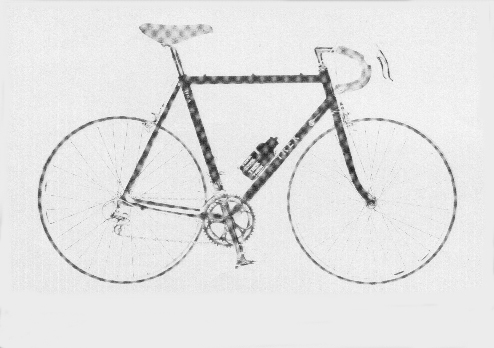
\includegraphics[width=0.3\textwidth]{frame}}\quad
	\subfloat[Frame FEA model]{\label{bike_fea}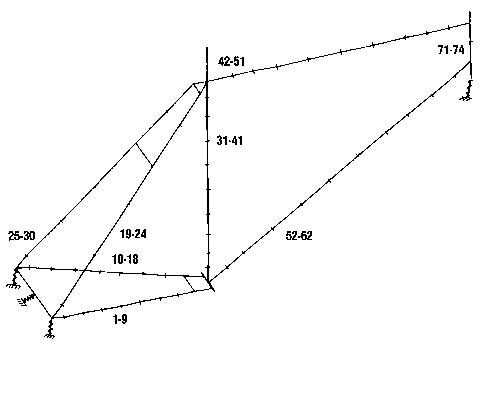
\includegraphics[width=0.3\textwidth]{frame_fea}}\quad
	\subfloat[Frame DOFs]{\label{bike_dofs}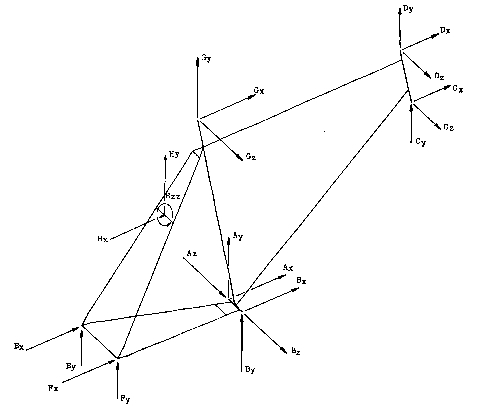
\includegraphics[width=0.3\textwidth]{frame_dof}}
	\caption{Example bicycle frame and corresponding FEA implementation}
	\label{frames}
\end{figure}
The FEA model is then used to run analyses to determine how the frame will perform under various loading conditions relating to typical operation.  These operation modes include:
\begin{itemize}
	\item{Static start-up (\emph{maximum effort applied to acceleration from a standing stop})}
	\item{Horizontal impact (\emph{reflects a low speed, head-on collision})}
	\item{Vertical impact (\emph{can be used for vibrational analysis or to study the effects of dropping})}
	\item{Front wheel braking (\emph{case when only the front brake is applied})}
	\item{Rear wheel braking (\emph{case when only the rear brake is applied})}
	\item{Steady state pedaling}
\end{itemize}

\subsection{FEA analysis of the wheel assembly}
\begin{figure}[h]
	\centering
	\subfloat[Thirty-six spoke wheel geometry]{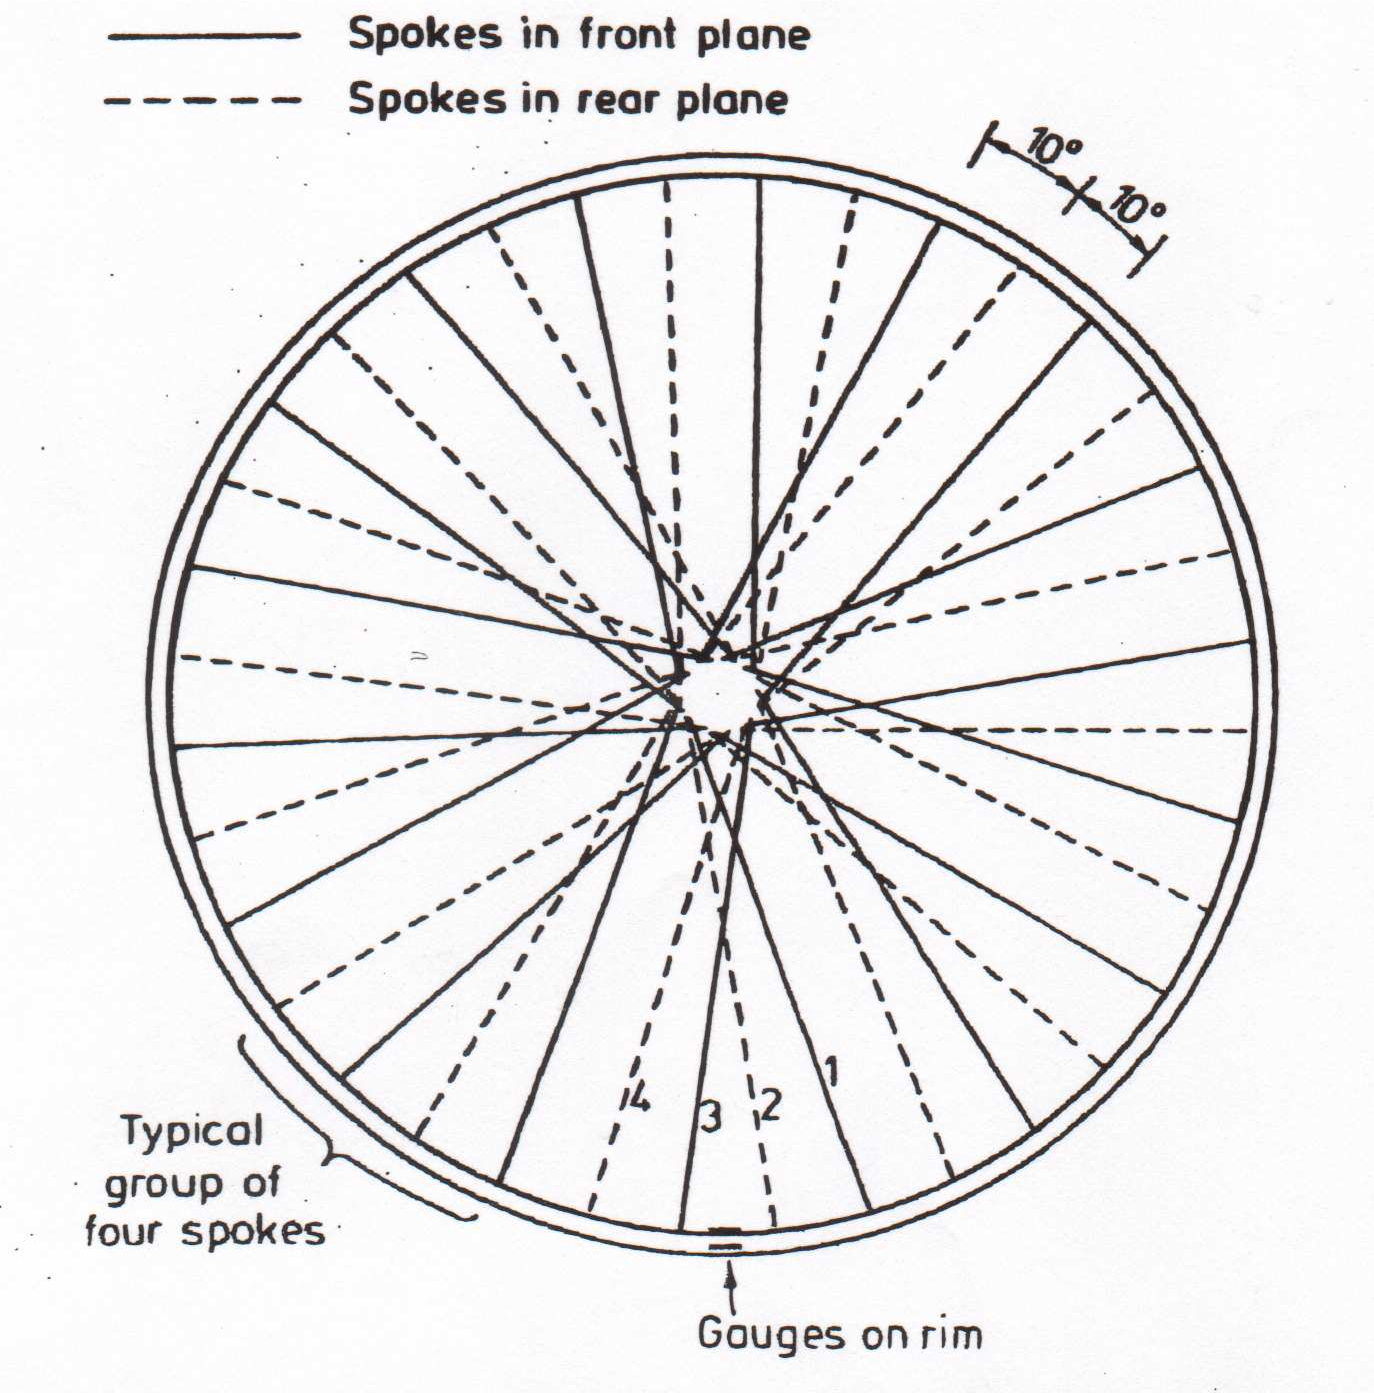
\includegraphics[width=0.3\textwidth]{wheel_geometry}}\quad
	\subfloat[Spoke geometry]{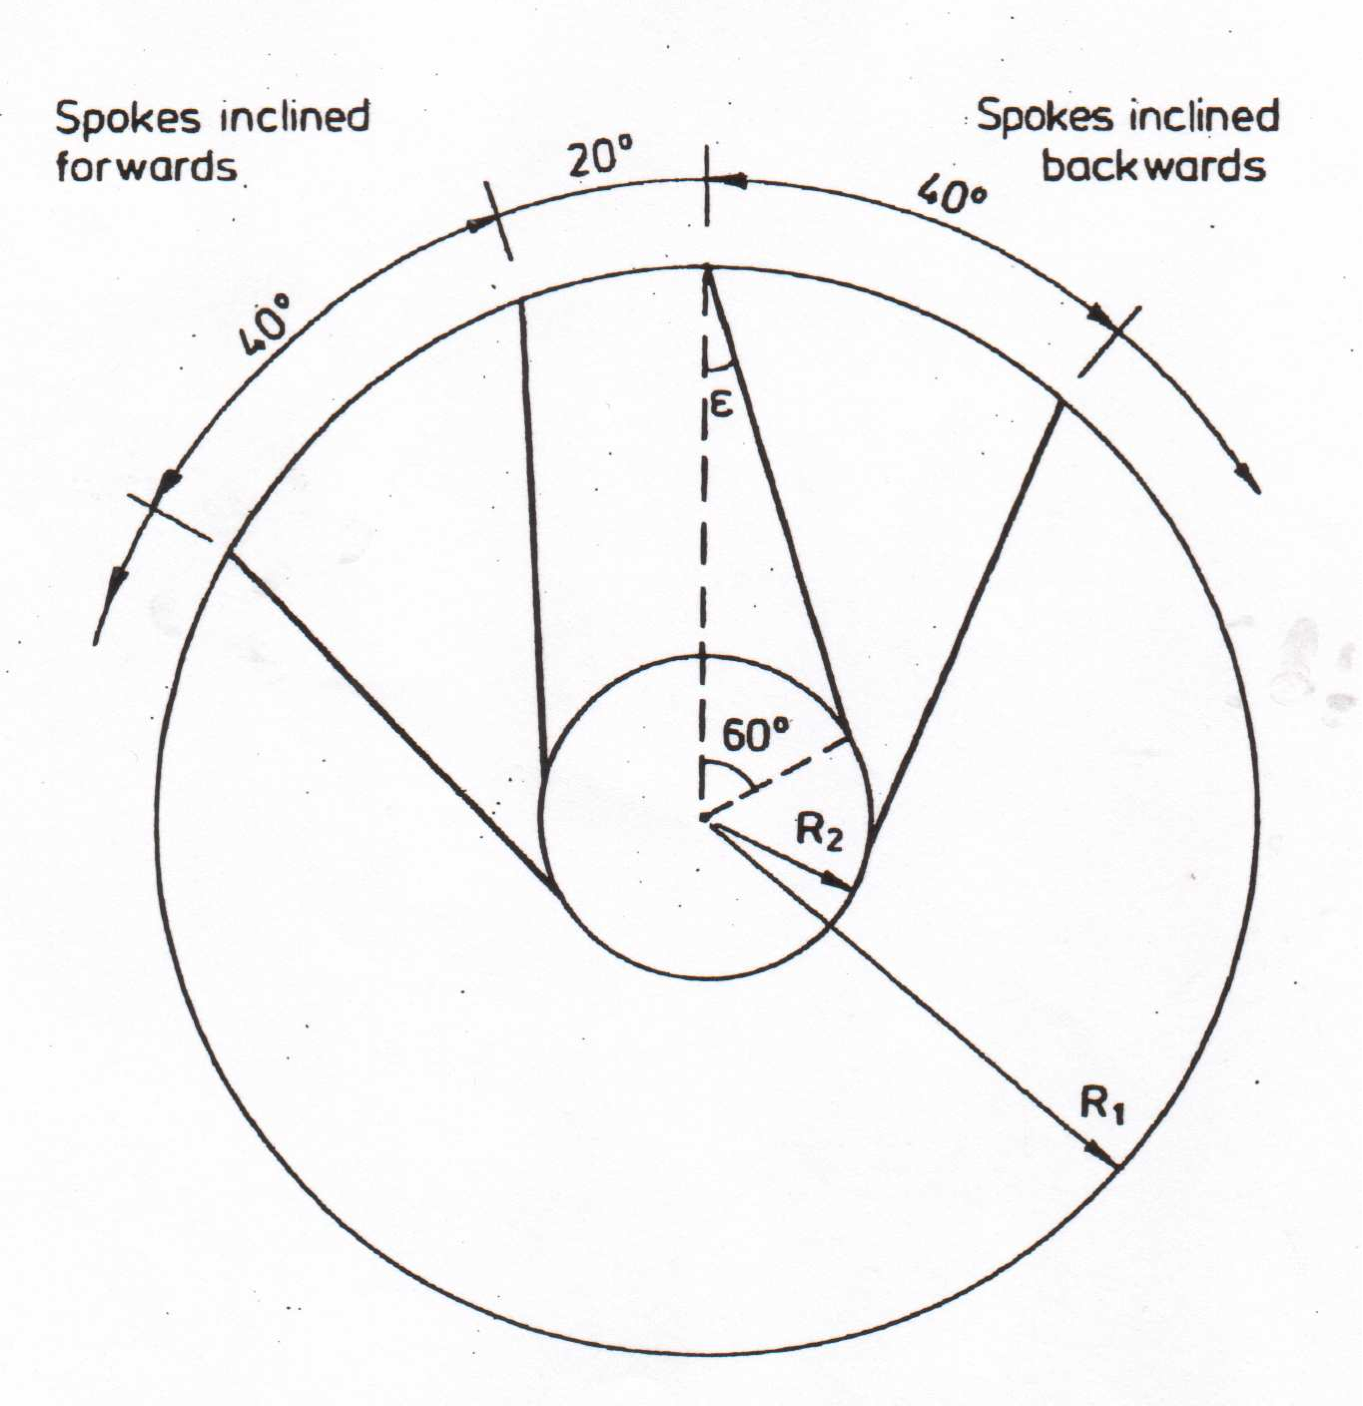
\includegraphics[width=0.3\textwidth]{spoke_geometry}}\quad
	\subfloat[FEA model]{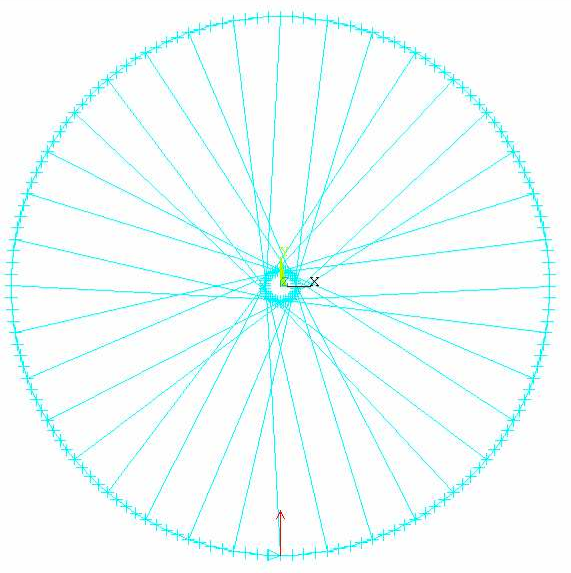
\includegraphics[width=0.3\textwidth]{wheel_fea}}
	\caption{Bicycle wheel geometry, spoke geometry, and corresponding FEA model}
\end{figure}

\subsection{Aerodynamic improvements}
Use of FEA in aerodynamic improvements to the bicycle, its components, and sometimes the rider's position is a relatively new development in bicycle design, mostly due to advances in materials and available construction techniques, such as hydroforming.  These advances allow bicycle manufacturers to very precisely construct frames and other large components aerodynamically, thus cutting down on drag, and therefore increasing the efficiency of the bicycle.  Additionally, aerodynamic improvements can also be found by using computational fluid dynamics in conjunction with the FEA analysis of the bicycle frame in order to optimize the rider's position while increasing the rigidity of the frame.  Due to the proprietary nature of this CFD analysis, no public domain work is available for review.  However, Felt Bicycles is one of the most prolific users of CFD in the design work of their frames, and they are famous for developing the one of the first competition legal aerodynamically designed bicycle frames (additional information about Felt's CFD analysis can be found online at \url{http://feltbicycles.com/USA/Single-Nav/Inside-Felt/Technology/Aero-Science.aspx}).

\section{Safety Analysis}

\section{Comments}


\end{document}